\section{Use case: Dental images}

\begin{frame}{\secname}{Problem description}
    In the context of dental health, as teeth are bones, the dentist needs to take X-rays.
    \begin{figure}
        \centering
        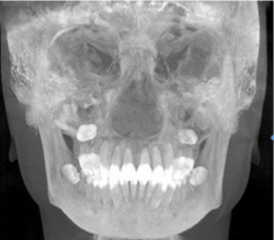
\includegraphics{img/dental_problem}
        \caption{Some teeth hide others \cite{yun_automatic_2019}}
    \end{figure}
\end{frame}

\begin{frame}{\secname}{Proposed solution}
    Yun \textit{et al}. \cite{yun_automatic_2019} came up with a solution based on the contents of this subject.
    \begin{figure}
        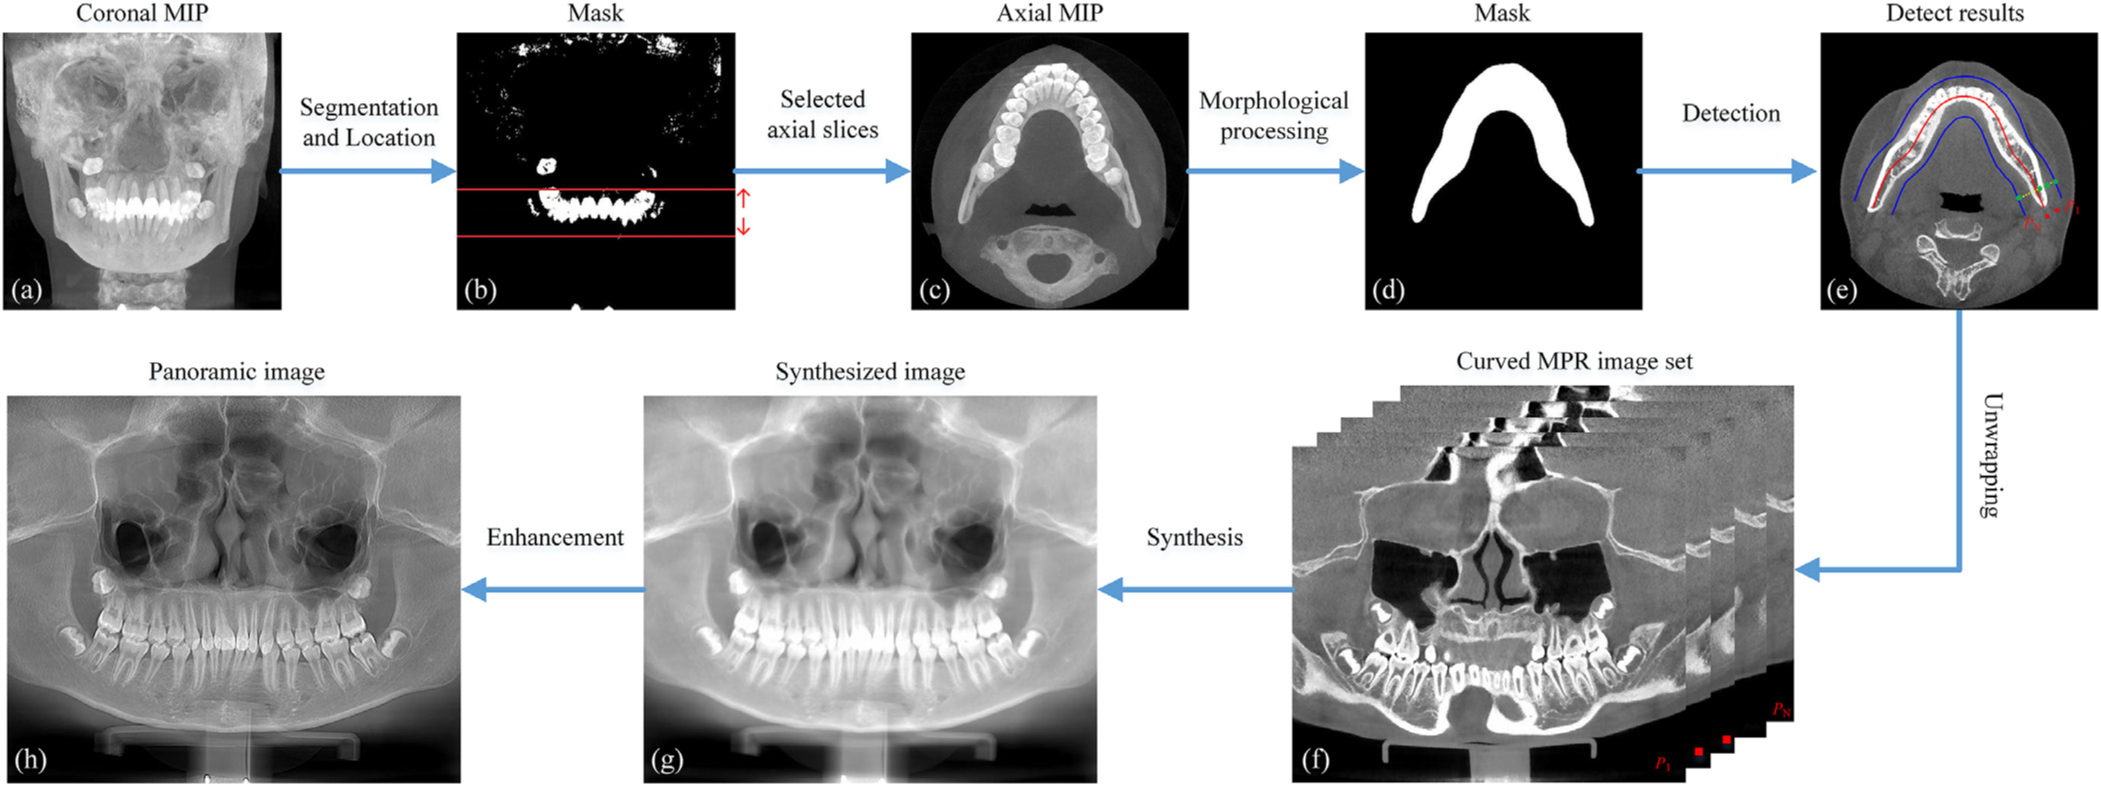
\includegraphics[width=\textwidth]{img/dental_proposal}
    \end{figure} 
\end{frame}

\begin{frame}{\secname}{Thresholding}
    They use histograms to establish a threshold value.
    \begin{figure}
        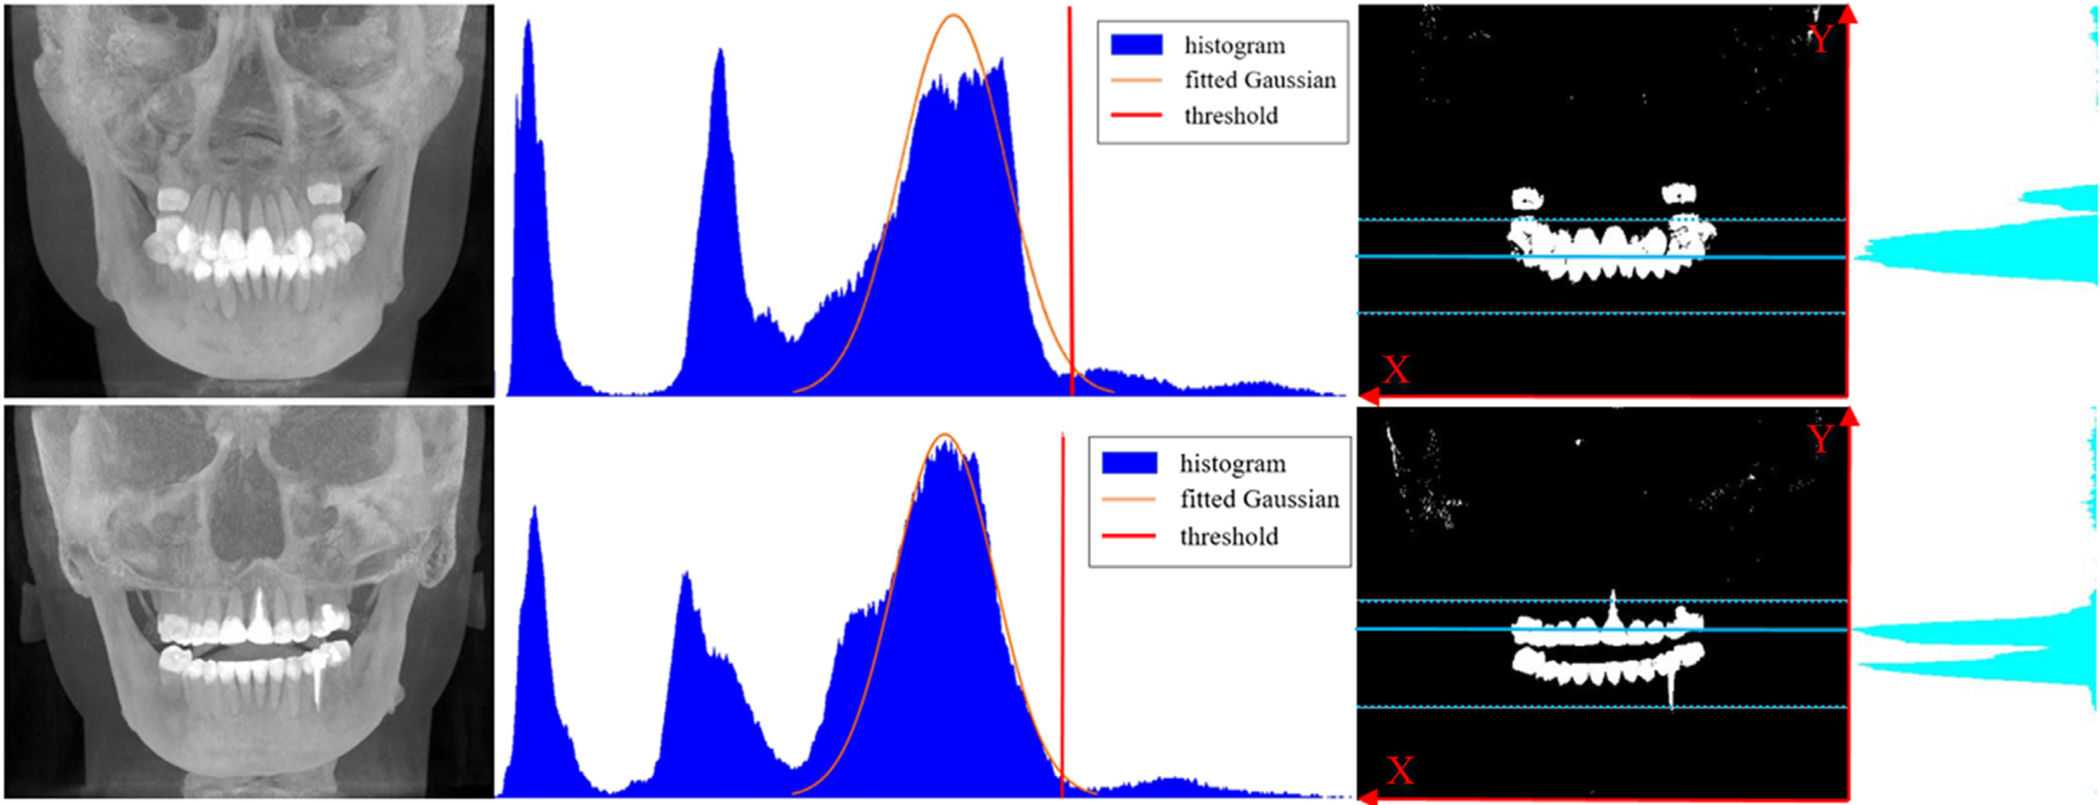
\includegraphics[width=\textwidth]{img/dental_thresh}
    \end{figure} 
\end{frame}

\begin{frame}{\secname}{Morphological processing}
    With the threshold calculated before, they managed to create a mask.
    \begin{figure}
        \centering
        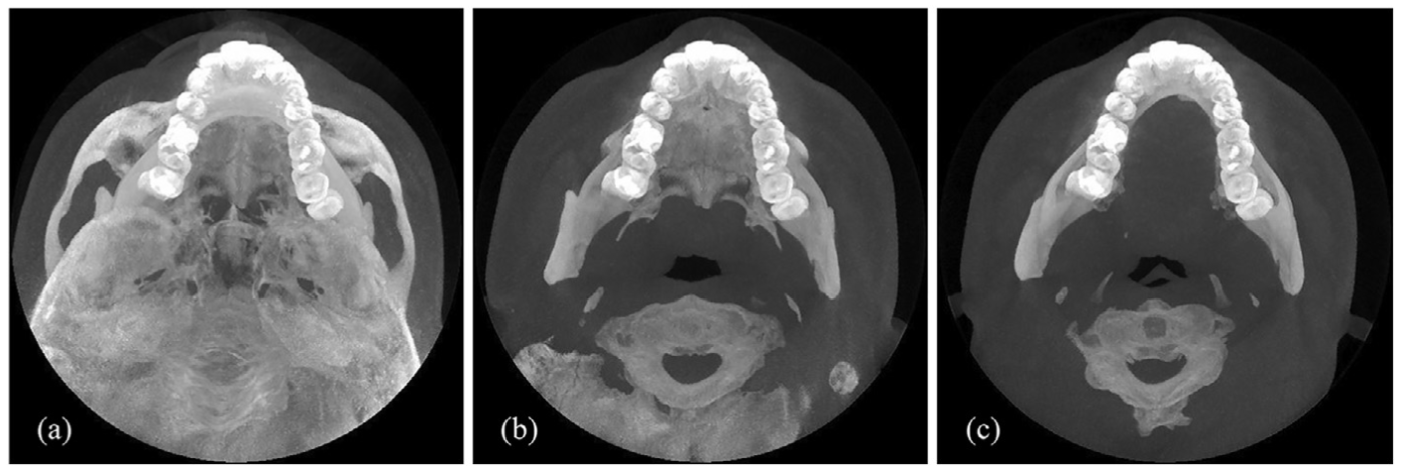
\includegraphics[width=0.7\textwidth]{img/dental_slices}
    \end{figure}
\end{frame}

\begin{frame}{\secname}{Morphological processing}
    With the threshold calculated before, they managed to create a mask.
    \begin{figure}
        \centering
        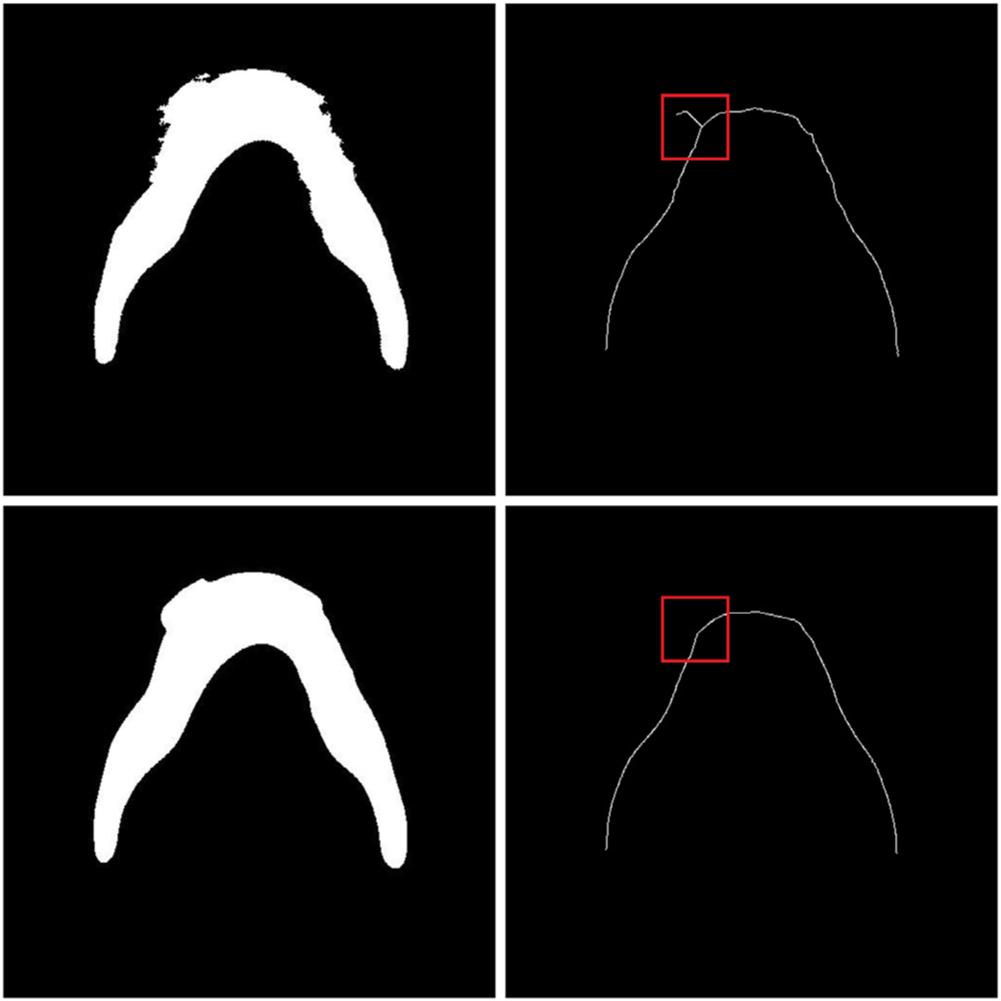
\includegraphics[width=0.3\textwidth]{img/dental_slice_thresh}
    \end{figure}
    Also perform Gaussian filtering
\end{frame}

\begin{frame}{\secname}{Arch approximation}
    Dental arch approximation using the following formula:
    \begin{gather*}
        I_0(i, j) = S \cdot \log \left( \sum_{n=1}^N e^{\frac{P_n(i,j)}{S}} \right)
    \end{gather*}
\end{frame}

\begin{frame}{\secname}{Arch approximation}
    Dental arch approximation are quite accurate:
    \begin{figure}
        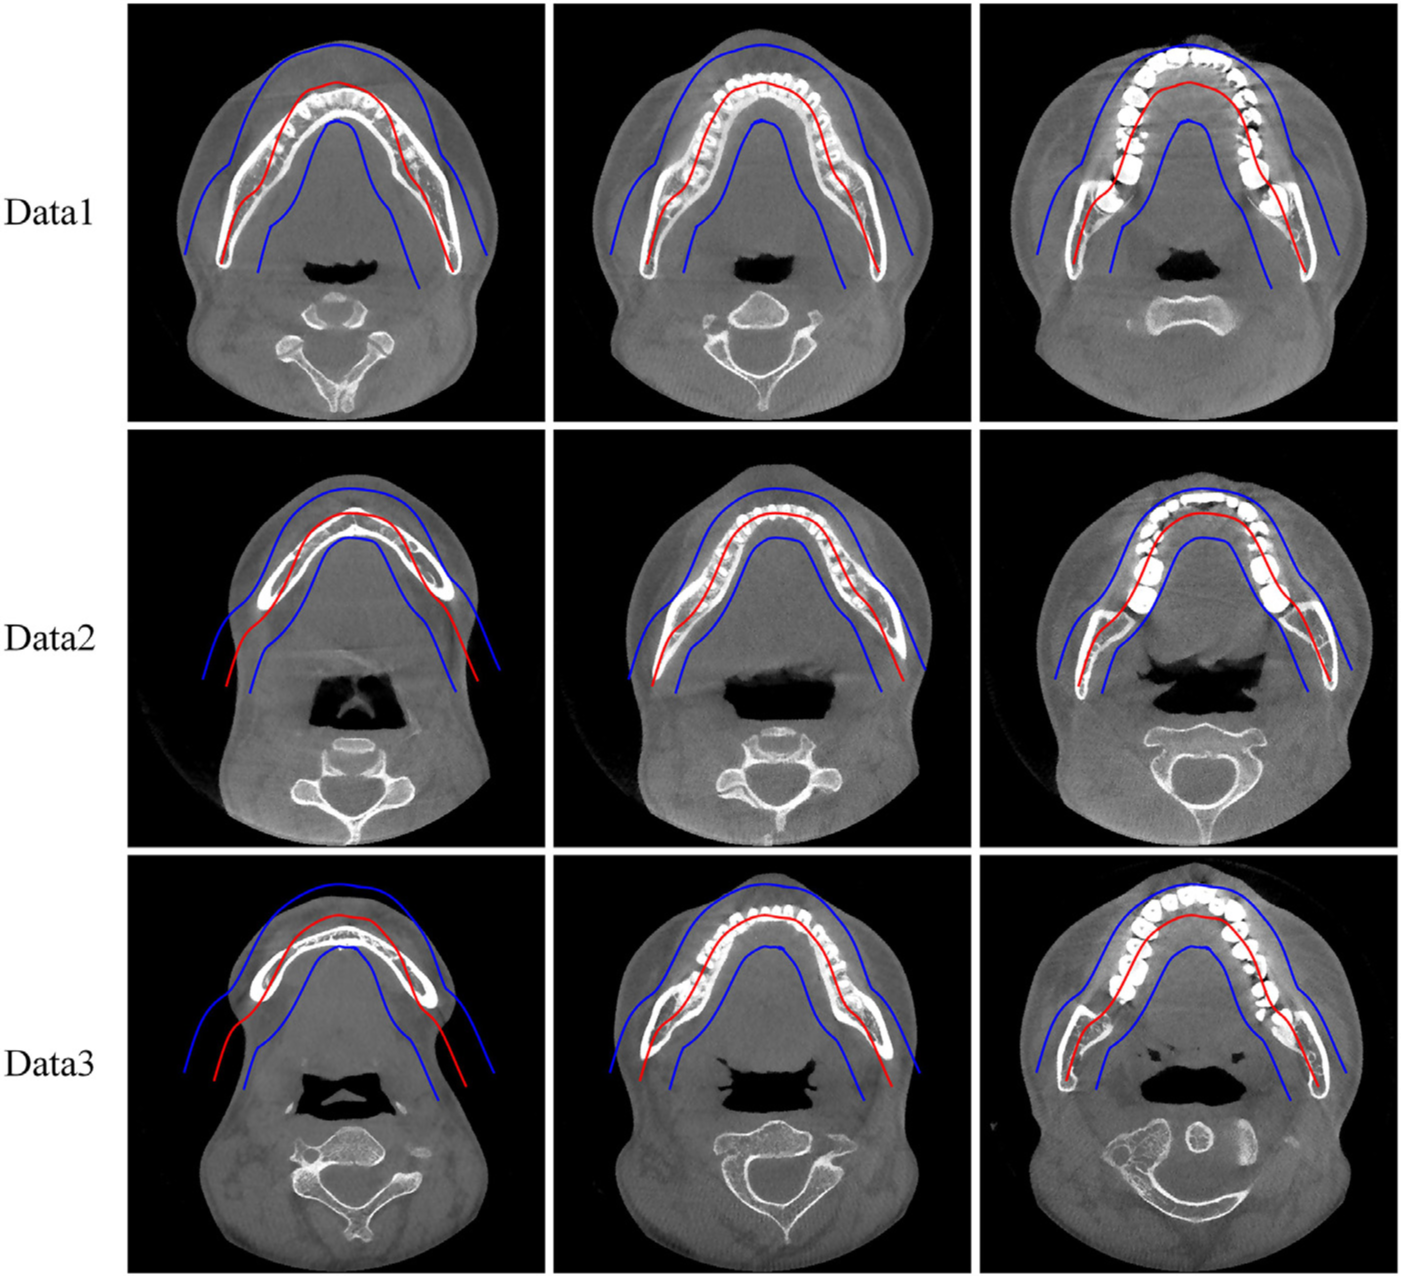
\includegraphics[width=0.7\textwidth]{img/dental_arch.png}
    \end{figure}
\end{frame}


\begin{frame}{\secname}{Panoramic images generation}
    Using homographies and the arch estimation in each tooth, they are able to reconstruct a panoramic image of the whole teething.
    \begin{figure}
        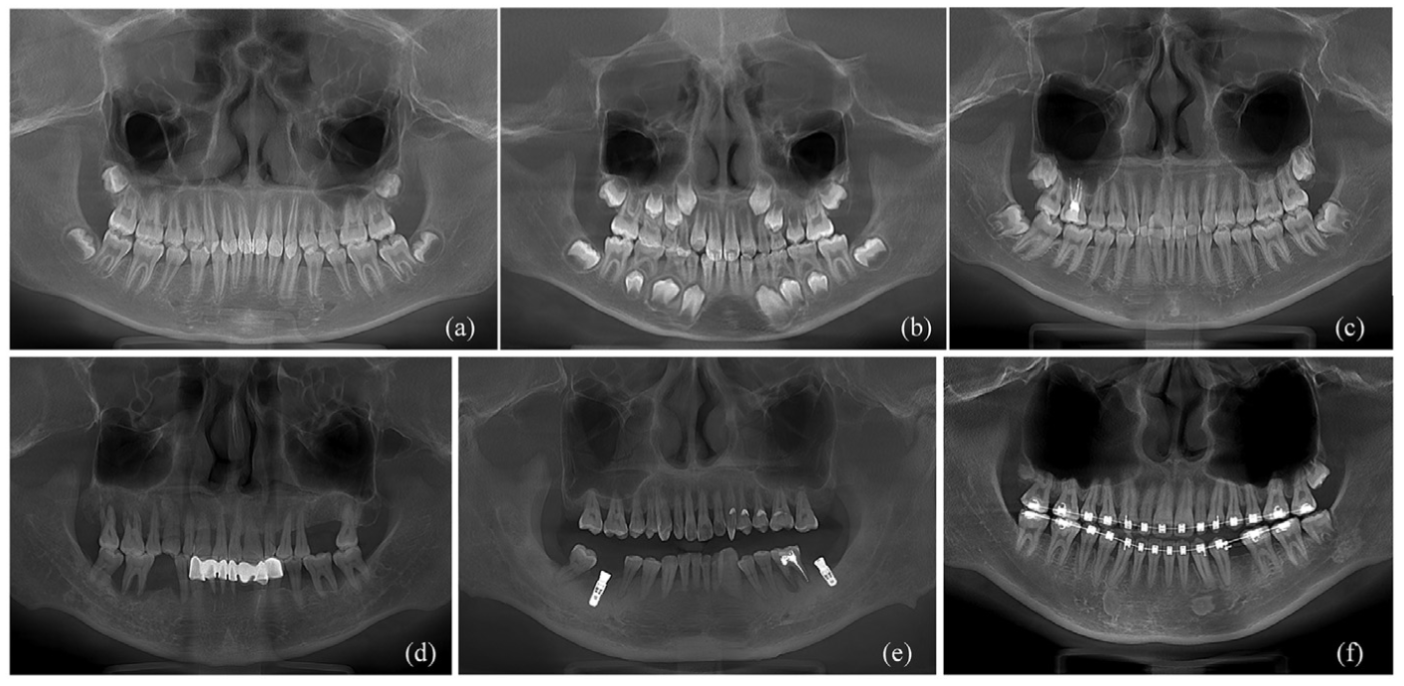
\includegraphics[width=\textwidth]{img/dental_pano}
    \end{figure}
\end{frame}

\begin{frame}{\secname}{Applications}
    Using techniques similar as the ones seen during the lessons, dentists can obtain automatic tooth identification.
    \begin{figure}
        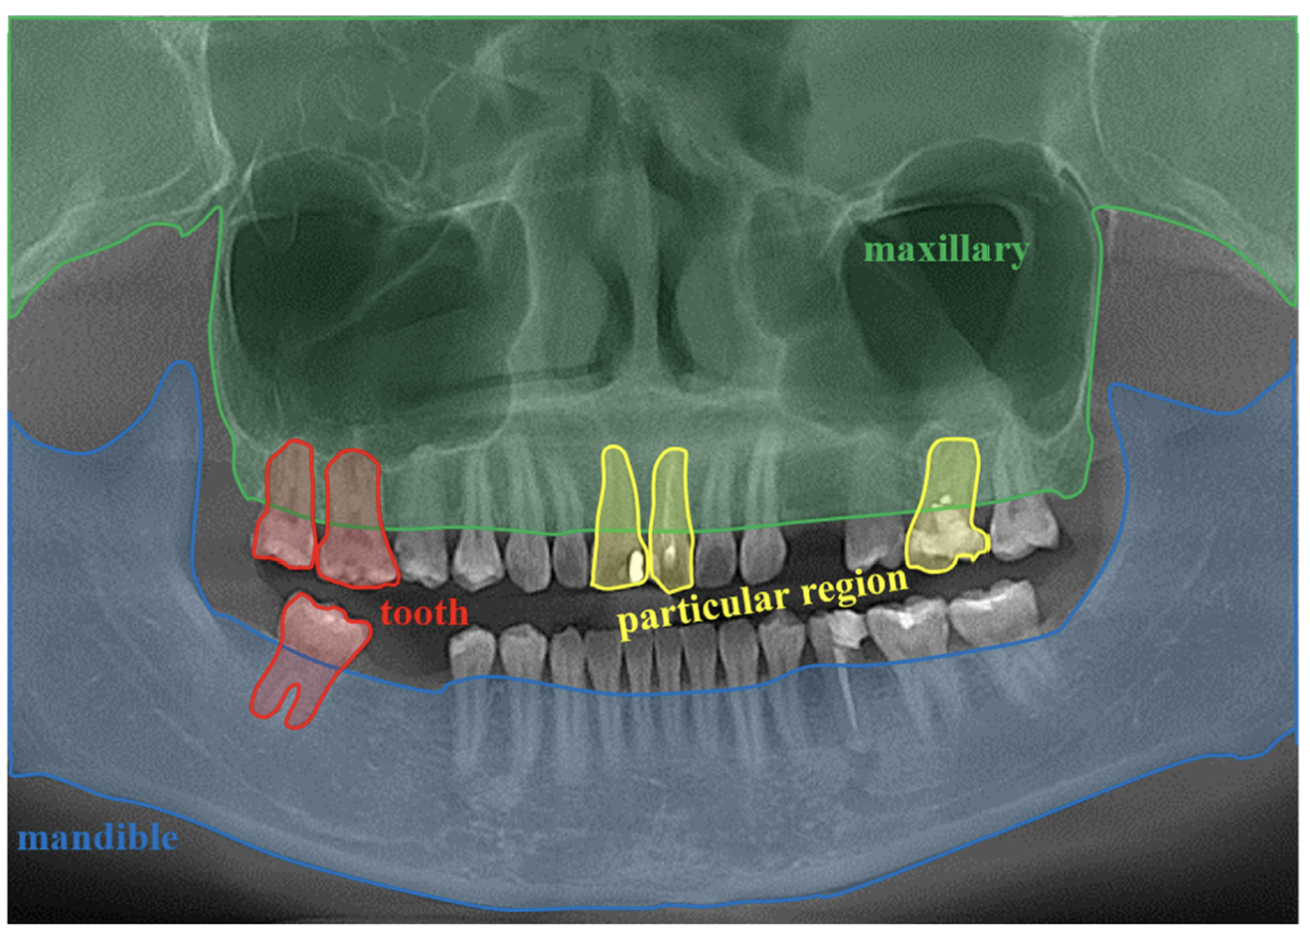
\includegraphics[width=0.5\textwidth]{img/dental_segmentation}
    \end{figure}
\end{frame}

\begin{frame}{\secname}{Known problems}
    One future path of this method is dealing with mental objects.
    \begin{figure}
        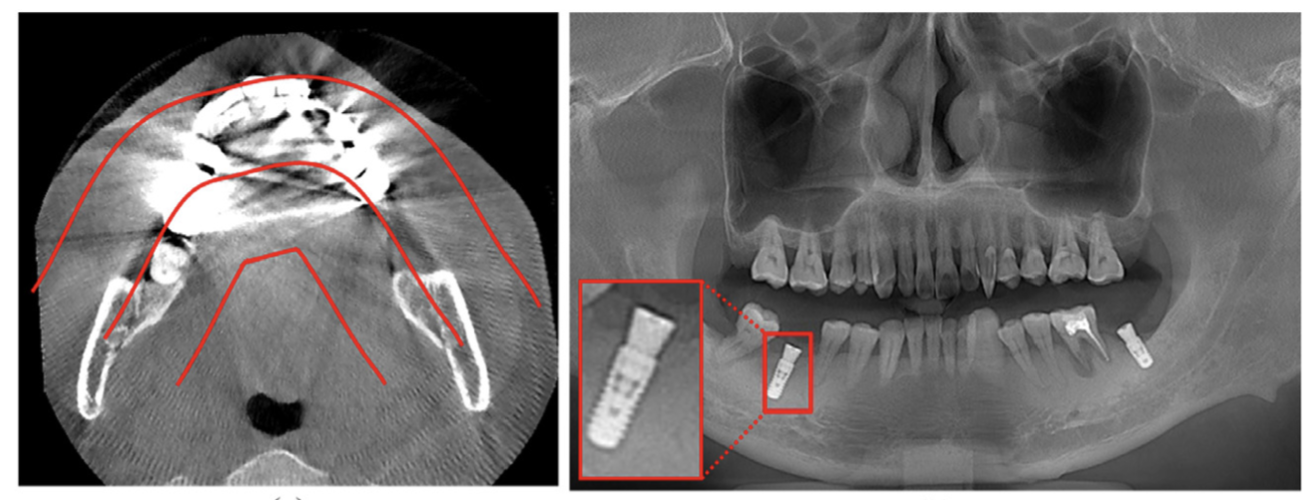
\includegraphics[width=0.7\textwidth]{img/dental_method_problems}
    \end{figure}
\end{frame}
